\chapter{Analyses} % Main chapter title

\label{Chapter:Analyses}

As presented in Figure \ref{fig:sustainableCityFramework}, the indicators for measuring a sustainable city are categorised into economic, social and environmental. This section of the report links the relation between urban agriculture and sustainable cities with reference to the indicators under each of the dimensions.

\section{Urban agriculture and economic sustainability of cities}
\label{sec:economicDim}

\subsection{Full-time employment}

Urban agriculture provides employment, and has become a means of a style-of-life, for people in cities particularly in the global south \cite{Kodjo2014, Zezza2010}. An estimated two thousand one hundred farm labourers in Morogoro and six thousand four hundred in Mbeya, Tanzania are involved in urban agriculture \cite{InternationalLabourOrganization2006}. In the same way, approximately a hundred twenty thousand low-income households in Manila, Philippines depend on the local/urban jasmine production for their livelihoods \cite{IPC2007}. Urban agriculture's role in employment creation abound in literature \cite{Amponsah2016}. See Table \ref{tbl:peopleEngagedInUA}.

\begin{table}[th]
\caption{Number of people engaged in urban agriculture in the global south. \cite{FAO2003}.}
\begin{center}
\begin{tabular}{ p{0.20\textwidth} p{0.25\textwidth} p{0.45\textwidth} } 
\hline
Region & Number (million) & Principal live-hood \\
\hline
Sub-Saharan Africa & 11 & Commercial vegetable growing or dairy farming \\
Northern Africa and the Middle East region & 6 & Horticultural and livestock products (fruit, vegetables and poultry) \\
South Asia & 11 & Perishable high-value commodities such as milk and fresh vegetables \\
East and South-East Asia & 7 & Perishable high-value commodities such as milk and fresh vegetables \\
\hline
\label{tbl:peopleEngagedInUA}
\end{tabular}
\end{center}
\end{table}

Urban agriculture is a source of employment to farmers but it is also to stakeholders in the supply chain, see Figure \ref{fig:vegySupplyChain}. The community of farmers and delivers in Argentina, Brazil and Uruguay are examples of jobs created in the commercial sector by urban agriculture \cite{InternationalLabourOrganization2006}. In the same way, most vegetable farmers in urban Ghana deliver their produce to wholesalers, who are predominately women \cite{Amponsah2016a, Amoah2007}. These wholesalers in turn sell the produce to retailers, food vendors and households as depicted in Figure \ref{fig:vegySupplyChain}.

\begin{figure}[th]
\centering
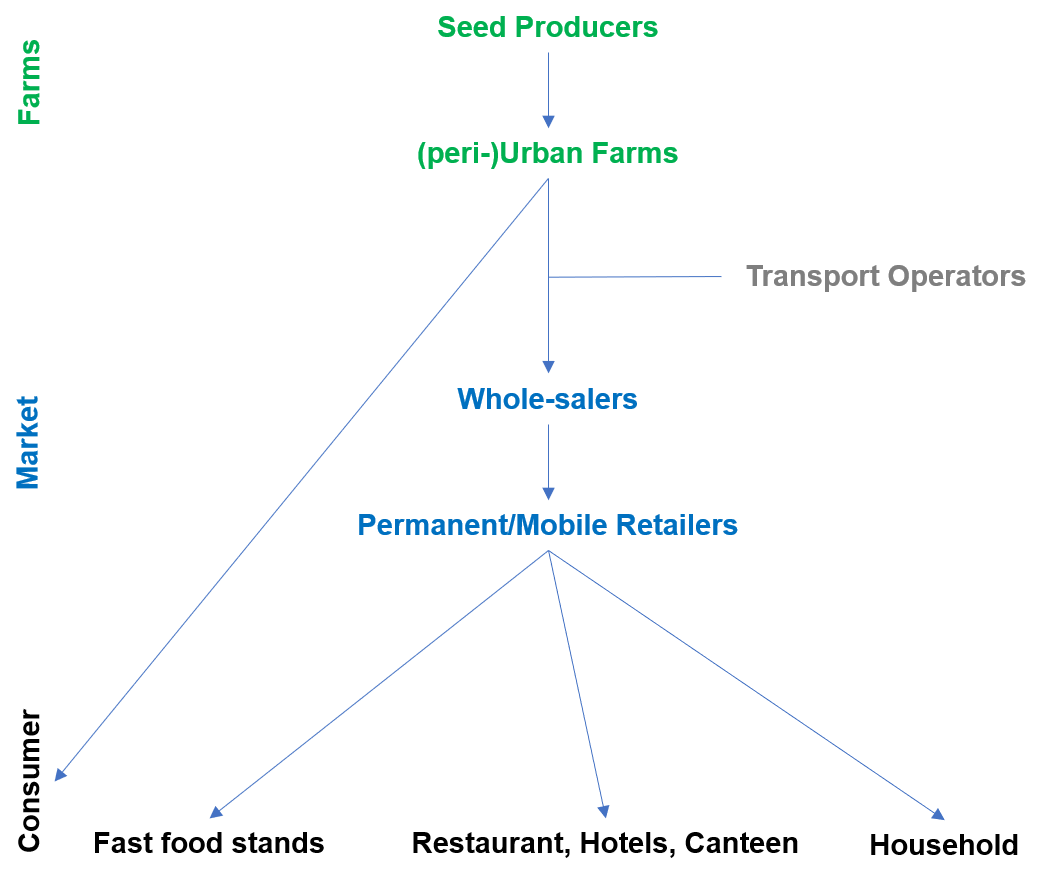
\includegraphics[width=0.75\textwidth]{./Figures/vegySupplyChain.png}
\decoRule
\caption[Flow chart of vegetable supply chain]{Flow chart of vegetable supply chain. \cite{Drechsel2014}}
\label{fig:vegySupplyChain}
\end{figure}

Urban agriculture has a significant contribution to the employment of the members of a city in the southern globe. In the cities in the global north, the motivation for authorities to stimulate agriculture in these cities is due to the ecological functions as well as the support for recreation areas \cite{Pearson2010}. Urban agriculture in the northern globe is not economically-centred but in its environmental functions. Nonetheless, recent studies state that urban agriculture in the global north is gradually shifting from leisure to urban sustainability \cite{McClintock2010}.

\subsection{Employment for women}

Prain and Lee-Smith \cite{Prain2010} state that two of three urban farmers in Yaounde, Nakuri, Maputo, Nairobi and Kampala are women. Typically, these women farmers engage in farming with the goal of providing their family needs of nutritious, chemical-free and fresh food \cite{Gamhewage2015}. Urban women farmers also sell the excess produce for income. Nevertheless, agriculture could be a bad thing to these women as they perform many tasks at the household. \cite{Veenhuizen}. Therefore, a conscious effort by policy makers and social advocates is required to minimise the workload on women from the combination of household errands and economic activities in urban agriculture.

Generally, commercial urban agriculture is dominated by men as described in Table \ref{tbl:genderinUA}. However, women are more present in the food market \cite{Drechsel2014}. It can therefore be deduced that commercial agriculture in the cities in the global south is gendered and thus makes a significant contribution to employment for both genders.

\begin{table}[th]
\caption{Gender in urban agriculture in selected cities. \cite{Amoah2007}}
\begin{center}
\begin{tabular}{ p{0.20\textwidth} p{0.40\textwidth} p{0.15\textwidth} p{0.15\textwidth} } 
\hline
Country & City & Female (\%) & Male (\%) \\
\hline
Benin & Cotonou & 25 & 75 \\
Burkina Faso & Ouagadougou & 38 & 62 \\
Cameroun & Yaoundé & 16 & 84 \\
Cote d'Ivoire & Abidjan/Bouake & 5-40 & 60-95 \\
Gambia & Banjul & 90 & 10 \\
Ghana & Accra, Kumasi, Takoradi and Tamale & 10-20 & 80-90 \\
Guinea & Conakry, Timbi-Madina & 70 & 30 \\
Mali & Bamako & 24 & 76 \\
Mauritania & Nouakchott & 15 & 85 \\
Nigeria & Lagos/Ibadan & 5-25 & 75-95 \\
Sierra Leone & Freetown & 80-90 & 10-20 \\
Togo & Tsévié, Lome & 20-30 & 70-80 \\
India & Delhi, Mumbai, Chennai, Hyderabad and Bengaluru & 17 & 83 \\
\hline
\label{tbl:genderinUA}
\end{tabular}
\end{center}
\end{table}

\subsection{Income generation and gross domestic product}

Households in developing countries accept urban agriculture as a source of livelihood \cite {Amoah2007}. Drechsel and Keraita \cite{Drechsel2014} state that two of three urban vegetable farmers in Accra, Ghana had no intentions of leaving the their job even if they were offered regular salaried employment. Amponsah et al. \cite{Amponsah2015} conclude that vegetable farming in Kumasi, Ghana, had become an employment decision for many citizens.

Amponsah et al. \cite{Amponsah2015} conclusion is due to the high incomes the farmers have from agricultural activities within the cities. For instance, Keraita, Jiménez, \& Drechsel Keraita2008 concluded that urban farmers in Ghana earned twice as much as their counterparts in rural areas. The increase in income appears to be present in several other cities in the global south as indicated in Table \ref{tbl:incomesByUfarmens}. The earnings enable the urban farmers to contribute to the national income. For instance, YiZhang and Zhangen \cite{YiZhang2000} found that 2.7 million urban farmers contributed 2\% of Shanghai's gross domestic product. Similarly, para grass production and sale in Hyderabad, India contributes an estimated annual income of 4.5 million USD to the city's economy. In Hartford, USA, urban agriculture is estimated to contribute between 4 and 10 million dollars in gross domestic product \cite{Nugent2000}.

\begin{table}[th]
\caption{Incomes earned by urban vegetable farmers in six cities. \cite{Keraita2008, Drechsel2014, Buechler2005}}
\begin{center}
\begin{tabular}{ p{0.30\textwidth} p{0.30\textwidth} p{0.30\textwidth} } 
\hline
City & Annual income per ha (US\$) & Annual GNI per capita (US\$) \\
\hline
Nairobi in Kenya & 1770 & 645 \\
Dakar in Senegal & 2234 & 773 \\
Kumasi in Ghana & 420-1920 & 522 \\
Hyderebad in India & 830-2800 & 771 \\
Haroonabad in Pakistan & 840 & 931 \\
Guanajuato in Mexico & 1935 & 7755 \\
\hline
\label{tbl:incomesByUfarmens}
\end{tabular}
\end{center}
\end{table}

The value of urban agriculture to a city's gross domestic product may not be significant when compared to non-agricultural land uses. This could be a reason for the pricing out of agriculture in city land use planning processes. Nevertheless, gross domestic production and other economic indicators underestimate the actual contribution of urban agriculture to city. The approach excludes ecological and social dimensions of urban agriculture. Probably, if these dimensions could be valued and added to the value of urban agriculture, then urban agriculture could be as valuable as other land uses.

\subsection{Savings and expenditure}

It can be observed from Table \ref{tbl:expenditurePattern} that expense on food in Bangalore, Accra and Nairobi for households who engaged in urban agriculture is below the average of 50–70\% for the urban areas \cite{FAO2003}. The cities in the northern globe, households spend minimum proportions of their incomes on food, which implies limited contribution of urban agriculture to household savings. The savings may however originate from transportation. The literature indicates that households spend less on transport to obtain or transport food as compared to the other household items. Hamilton et al. \cite{Hamilton2014} had observed that savings occurred as a result of the reduction in transport cost for the urban farmer. The savings result from the amount these farmers would have otherwise incurred if they were to travel to procure the items, they produce themselves. moreover, urban agriculture allows farm produce to be closer to consumers than if the produce is to be supplied by rural farmers. This will therefore reduce travel cost and time to access food items by urban households.

\begin{table}[th]
\caption{Expenditure pattern of urban agriculture households in some selected cities. Source: World Bank (2013).}
\begin{center}
\begin{tabular}{ p{0.30\textwidth} p{0.20\textwidth} p{0.20\textwidth} p{0.20\textwidth} } 
\hline
Expenditure item & Selected cities &  &  \\
  & Bangalore & Accra & Nairobi \\
\hline
Food & 29.2 & 36.5 & 39.4 \\
Utilities & 16.8 & 12.3 & 13.1 \\
Education & 11.5 & 16.7 & 16.9 \\
Health & 10.4 & 8.2 & 5.1 \\
Clothes & 8.1 & 7.7 & 3.0 \\
Shelter & 7.0 & 3.2 & 18.9 \\
Loan/debt & 6.2 & 1.4 & 0.4 \\
Transport & 4.6 & 7.9 & 2.5 \\
Other & 3.3 & 0.8 & 0.2 \\
Family events & 2.1 & 4.5 & 0.2 \\
Domestic help & 0.7 & 0.8 & 0.2 \\
\hline
\label{tbl:expenditurePattern}
\end{tabular}
\end{center}
\end{table}

%\subsection{Tax revenue}
%
%Taxes are very important elements in managing developmental activities in cities. Taxes collected through urban agriculture covers all the actors along the produce supply chain. It is worth noting that, national income from taxes from urban agriculture can be directly linked to the expenditure farmers make and the employment obtained. Urban agriculture contributes significantly to tax revenues from property taxes. According to Liu \cite{RIZWAN2008} and Voicu and Been \cite{Voicu2008}, urban farms and community gardens contribute to the increase in home values. For instance, the presence of gardens in California contributed to the rise in property values as much as 9.4\% within five years of establishment \cite{Voicu2008}. The revenues were estimated at half a million dollars per garden over twenty years.
%
%Transportation taxes are also paid by urban farmers who transport their goods within or outside the urban area. Some urban farmers indirectly pay transportation taxes through the purchase of fuel for irrigation or the transportation of farm goods and services. Additionally, the wholesalers or retailers engaged in the sale of the urban agricultural produce pay taxes to city authorities. In Kumasi, a city in Ghana, wholesalers and retailers who operate in the open markets pay taxes in the form of market tolls (tickets) \cite{Baah-Ennumh2012}. The amounts paid ranges from 5 to 10GHp (0.01 USD–0.02 USD) a day and are paid to the Kumasi Metropolitan Assembly. Similarly, in the United States, the income that is obtained from urban farming does not represent a separate kind of income. They are determined and taxed like income from other businesses of a comparable size apart from some detailed regulations regarding farm income. However, national subsidies for soil, groundwater or environmental protection, care for wild animals or forests are sometimes tax-free for the farmers \cite{Andersen2002}. In a similar vein, some municipalities (Rosario in Argentina and Cagayan de Oro in The Philippines) use tax exemptions as a means of promoting urban agriculture.
%
%Useful as the taxes may be, taxes to the cities may be more if the agricultural lands had been used for non-agricultural purposes such as commerce or industry. The tax exemptions could also be avoided if the lands were used for non-agricultural purposes. Such arguments are underpinned by the theory of ‘highest and best use’ which focuses on only the direct economic benefits derived from the use of land. These theories suggest that allocating land for urban agriculture deprives its access for other more economically beneficial uses such as industrial, commercial and residential uses. This explains why a rise in the value of urban agricultural land is mostly associated with the change in use from agriculture to alternative land uses \cite{Nugent2000}.

\section{Urban agriculture and social sustainability of cities}
\label{sec:socialDim}

\subsection{Educational functions}

Buehler \cite{Buehler2016} states that urban agriculture allows a means for learning experiences, youth development and educational programmes. Agricultural projects in California and Philadelphia, USA, are implemented to show the role of urban agriculture in education \cite{Bradley2014}. These educational services are directed towards teaching the citizens the food-supply-chain of the products they eat, so as to enable them make informed decisions about their food selection.

Moreover, through social networks, urban farmers who have had the benefits of education by research institutions, the knowledge is shared. Urban vegetable farmers in Kumasi in Ghana who have participated in research activities on the World Health Organization's Multiple Barrier Interventions have teach their counterparts who were not part of the training programme \cite{Amponsah2015, Amponsah2016}. This highlights the replication effects of such research projects on the larger community.

Urban farmers' earnings from agriculture are used to support their children in school \cite{Prain2010}. A study in SriLanka by Gamhewage et al. \cite{Gamhewage2015} states that 22\% of urban farmers prefer to expend their savings on the education of their children to spending on household possessions. Similarly, in India, some women contribute approximately 23\% of their share in household education expenditure from the incomes they earn from urban agricultural activities. Another study in Kampala, Uganda also concluded that urban male farmers and female farmers spend 26\% and 12\% of their incomes respectively on the fees of their wards in school \cite{Buechler2005}.

However, urban agriculture in the global south is known to stimulate child labour and school deviation \cite{Edet2013, InternationalLabourOrganization2006}. For instance, in Dar-es-Salaam, Tanzania, children engage in urban agriculture at the expense of their education. Similarly, child migrants have been found to be engaged as farm labourers on urban farms in Kumasi, Ghana \cite{Amponsah2016a}. In spite of, in these countries, child labour is prohibited. The higher returns from the urban agricultural activities could be an explanation for their attractiveness to children. Children can take advantage of the primary educational policies and programmes in these countries to attend schools \cite{Nishimura2013}. This will enhance the educational functions of urban agriculture towards social sustainability of cities.

\subsection{Civic engagement}

Obach and Tobin \cite{Obach2014} and Pole and Gray \cite{Pole2013} conclude that people in New York City who were engaged in urban agriculture were more politically engaged and more likely to volunteer in their communities compared to the general population. In the same way, in Dar-es-Salaam in Tanzania, urban farms were used as political gathering spaces in during the 2010 elections. However, Pole and Gray \cite{Pole2013} state that the desire for organic foods is the motivation for people to interact with urban farmers other than civic engagement. Obach and Tobin \cite{Obach2014} conclude that consumers of urban agricultural products are less likely to engage in charitable giving than the general population. The studies conclude that if the motivation for engaging in urban agriculture is economic, then it is less likely to promote civic engagement.

The economic reasons including household food security, employment and income generation are the main motivations for people's engagement in urban agriculture \cite{Amponsah2016a, Kodjo2014, InternationalLabourOrganization2006, Zezza2010, Amoah2007}. Besides, the reasons for agriculture in the cities in the global north are more leaned towards leisure and ecological functions \cite{InternationalLabourOrganization2006, Hamilton2014}. Urban agriculture's role in civic engagement is more pronounced in the global north than the southern globe.

\subsection{Safety and security}

Urban agriculture provides a significant contribution to the safety of a city. Gardens help to promote energy efficiency in buildings and contribute to fire prevention \cite{Hoornweg2012}. Furthermore, clearing an area of bush in a city for agricultural purposes has the potential to eliminate hiding spaces for thieves. Interactions make profound contributions to the social sustainability of cities; as customers, people walking through, people who live nearby, people looking for a day labour job, and more, interact in urban farms.

The University of Pennsylvania's Perelman School of Medicine in Philadelphia executed a study and conclude that greening vacant lots made residents feel significantly safer, and that the greened lots lead to reductions in certain gun crimes in the area \cite{Krauser2012}. This is consistent with the work of Kuo \cite{Kuo2001} which stated that the greener a building's surroundings were, the fewer the reported crimes. Kondo conducted a study and stated that there were reductions in crime levels \cite{Kondo2016}. This could confirm that states that are maintaining and monitoring urban environments in a well-ordered condition may stop further vandalism and escalation into more serious crime. The Urban Food Crisis \cite{TheUrbanFoodCrisis2018} explains that using blighted lots for urban agricultural purposes reduces crime rates.

Other studies point to the negative side of urban green space \cite{Bixler1997}. These include encounters with physical danger such as poisonous animals and thorny plants, and the fear of crime \cite{Sreetheran2014}. These authors, after a systematic review of literature, point out, however, that factors such as gender and individual's experiences are most influential in evoking fear of crime. This means that the crimes that result from urban agriculture may be imagined from an earlier experience. A fear of crime may therefore be imagined but not real. People should be alerted to thorny plants and poisonous animals to mitigate the adverse effects on neighbourhoods. These measures could enhance the role of urban agriculture in urban safety and security.

%\subsection{Gender equality and social equity}
%
%Urban agriculture can close the gender gap and stimulates social equity through the employment opportunities it offers to both men and women. As presented earlier in Table 2, women form a significant part of the labour force that is engaged in urban agriculture. They can gain employment at every stage of the supply chain. This reduces gender inequalities \cite{InternationalLabourOrganization2006}. In the case of hired labour, more women (54\%) than men were employed. Kutiwa, Boon, and Devuyst \cite{Kutiwa2010} also point out that urban agriculture in Harare in Zimbabwe provides women the opportunity to earn secondary income, improve nutritional value of the household diets, and participate actively in budgeting and decisionmaking processes at the household level.
%
%However, women tend to engage in urban agriculture for household food supply while men engage in it for economic reasons. This could perpetuate the income gap between men and women in many cities. Furthermore, the disparity in the gender roles at the family level implies greater burden on women in the cities in the global south than men. Typically women shoulder more household responsibilities (like childcare and domestic work) than men \cite{Mencarini2012}, which implies that urban agriculture could have the potential to aggravate the burden of work on women and gender inequality \cite{Veenhuizen}. These have implications for the systems and practices that perpetuate gender inequality but not necessarily preventing a certain gender category from engaging in urban agricultural activities or any economic activities.

\subsection{Health benefits}

Urban agriculture enables an improvement to the health of a city through its contribution to food security \cite{Opitz2016} and income for farmers and their families to access health care. Community gardens give residents access to fresh fruits and vegetables \cite{Larsen2009}, which are essential to safeguarding their health. From a social point of view, urban agriculture can provide food availability and accessibility. Also, citizens can take advantage of the urban produce to diversify the food intake, which ultimately leads to healthier diets. Research also supports that people who participate or have family members that engage in community gardens “are 3.5 times more likely to consume fruits and vegetables at least 5 times per day than people without a gardening household member” \cite{Alaimo2008}. Urban agriculture helps to reduce malnutrition and promote the general health of the city population.

However, some studies point to the adverse effects of urban agriculture on the health of the cities. These studies stand out the excessive use of agro-chemicals \cite{Veenhuizen, Amoah2007, Agbenyour2014}, which could undermine the health of producers, consumers and the environment, and the use of untreated waste-water for food production \cite{Amponsah2015, Veenhuizen, Becerra-Castro2015, Amponsah2015, Mara2010, Ndunda}. Moreover, the urban agricultural farms can lead to the spread of diseases through mosquitoes and the scavenging animals. Due to these adverse effects, the emphasis of the discourse on the role of urban agriculture in cities' social sustainability should focus on responsible agriculture.

%\subsection{Recreation}
%
%Community gardens and rooftop gardens contribute to both indoor and outdoor recreation \cite{Hamilton2014}. These gardens can provide a place where people in an area in a city come together for mutual benefits. For instance, in the early 20th Century, upper class Russians resorted to dachas as hobby farming to improve upon recreation \cite{Hamilton2014}. Community gardens and rooftop garden also serve as tourist attraction centres \cite{InternationalLabourOrganization2006} and improve the value of urban property. A classic example of this is in Beijing China. Here, people spend one-day to tour over 1900 sightseeing farms and pick produce \cite{InternationalLabourOrganization2006}.
%
%Some individuals in Detroit have resorted to urban agriculture as a means of increasing the value of their property \cite{Walker2016}. Each community garden in California also contributed about half a million dollars to the local economy through rise in the value of real property \cite{Voicu2008}. People are attracted to some of these buildings because of the plants and ornaments around.
%
%\subsection{Technology and innovation promotion}
%
%Urban agriculture provides the avenue for the development of technology. For instance, some urban farms in Hong Kong Island, China are recycling water with PV-powered UV-LED disinfection \cite{Close2006}. Other farms use hydroponic \cite{Buehler2016} systems to produce leafy greens, tomatoes, and herbs. These technologies could contribute to the preservation of urban agriculture and its significant roles even in cities where land is increasingly becoming scarce due to rapid urbanisation.
%
%Urban agriculture also provides an avenue for new research and technology to be developed. Examples include research on varieties of seeds, and type and amount of light required for plant growth. This type of agriculture therefore incorporates the use of technology as a means of optimising levels of production. Disregarding technology and innovation in urban agriculture could result in unreliable and ineffective farms.

\section{Urban agriculture and environmental sustainability of cities}
\label{sec:environmentalDim}

\subsection{Management of emissions}

Cities are known for their poor air quality due to GHGs emissions from vehicles and industries \cite{Heather2012}. The cities are often with dangerous levels of greenhouse gases. Urban agriculture can manage of these emissions \cite{Padgham2015}. It is estimated that 711 thousand metric tons of air pollution is removed annually by urban trees \cite{Yang2008}. Nevertheless, in high dense populated urban areas, it is difficult to place enough trees to promote air quality; in that situations, rooftop gardens can be implemented.

Yang et al. \cite{Yang2008} conclude that the levels of acidic gaseous chemicals decreased by 37\%, on a 4 thousand $m_{2}$ green roof built in Singapore. Similarly, a study in Toronto, CA, calculated that 7.87 metric tons of air pollutants per year could be removed by 109 ha of green roofs \cite{Yang2008}. Planners and city authorities, particularly in the cities in the global north, are making conscious efforts to implement green infrastructure in their city planning processes. Canada, under the Ottawa Green Belt Programme, has acquired 37,000 acres of land for green infrastructural purposes, which includes urban and rural farming \cite{Pearson2010}.

Notwithstanding the urban agriculture ability to manage GHGs emissions, some authors argued that organic urban agriculture can result in the emission of some gases, which may cause negative effects to the environment. Davison and Cape \cite{Davison2003} conclude that about 90\% of atmospheric ammonia in the US come from organic agriculture, as the ammonia is generated from agricultural activities including soils, fertilisers and domesticated animals waste \cite{Paulot2014}. The ammonia is transported by winds and returns to the surface by wet or dry processes, which may contribute to the degradation of air quality and visibility, as well as to the atmospheric radiative balance \cite{Aneja2015}.

%\subsection{Water management}
%
%Sustainable water management in the radar of city authorities across the globe. Forecasts by the OECD (2012) estimate that over 40\% of the world's population will live in a water-stressed situation 2050. It is estimated that irrigated agriculture accounts for around 70\% of all the world's freshwater availability \cite{Rosegrant2009}. The implication is that irrigated urban agriculture can increase the pressure on available freshwater resources in the water-stressed areas in the globe. Consequently, the promotion of urban agriculture and the risk of fuelling the pressure on freshwater resources is in debate. The limited freshwater can be applied for non-agricultural purposes.
%
%Literature states that waste-water reuse, sheet mulching, and drip irrigation can reduce the pressure urban agriculture on freshwater resources \cite{Ensink2004}. In the same way, other irrigation techniques such as aeroponics, film farming \cite{Ayambire2019}, automated weather station networks, soil and plant measurement systems, and dynamic simulation models \cite{Itzhaky2010} can reduce the water scarcity pressure. The discussion points to the use of less costly options such as sheet mulching and wastewater for restricted irrigation.
%
%Wastewater treatment is ideal. However, the high wastewater treatment cost challenges its adoption in the low-income cities in the global south. In this regard, emphasis of the discourse should be on wastewater reuse for restricted irrigation \cite{Hamilton2014}, which calls for its promotion to resolve the negative perceptions urbanites have about wastewater reuse for productive purposes \cite{Mayilla2017}. Urban farmers and stakeholders along the value-chain should also be monitored to comply with health risks reduction measures (see WHO guidelines for the safe use of wastewater, excreta and greywater in agriculture) when using wastewater for restricted irrigation purposes. This will safeguard public health. Land tenure security could be an important strategy to encourage the commercial urban farmers, particularly in sub-Saharan Africa, to comply with the health risks reduction measures.

\subsection{Waste management}

Urban agriculture provides a means to put organic waste to good use. Due to the nutrient-rich properties, Germany encourages the use of solid waste as compost in agriculture. Other European Union member states are developing technologies to collect organic waste and produce compost for agricultural purposes \cite{Anastasiou2014}. A New York City study in 2009 stated that more than 130 urban gardens had composting processes, which were merged within the existing city sanitation processes. In the same way, the Governador Valadares provides incentives for composting and reuse of solid waste in urban farms; the City of Cape Town also provides incentives for the use of compost. \cite{Hoornweg2012}. The use of compost for crop farming in the cities in the global south has been extensively reported in the conventional literature \cite{Amoah2007}. These initiatives help to improve environmental sanitation.

Urban agriculture also positively affects the treatment of waste-water. Lydecker and Drechsel \cite{Lydecker2010} conclude that vegetable farms in Accra in Ghana treat the waste-water from about 225 thousand households. The soils serve as filters for the treatment of the waste-water that is used for irrigation purposes. On the other hand, Drechsel and Keraita \cite{Drechsel2014} estimate that urban farms can only absorb and filter a limited amount of the waste-water due to the high degree of pollution. Notwithstanding, agricultural lands have a significant role in reducing the environmental pollution that results from untreated waste-water into the environment. Pollution of the sea and other freshwater resources by untreated waste-water is reduced when it is used for irrigation purposes \cite{Liu2013}.

In spite of the promising features of urban agriculture in waste management, urban agriculture can lead to the discharge of waste-water into water bodies. Veenhuizen \cite{Veenhuizen} states that urban farms jettison waste-water into open water supplies. As a mitigating strategy, some cities (such as Harare in Zimbabwe) have adopted an approach to filter water from farms through a natural purification process before it enters the city reservoir \cite{Kutiwa2010}. Consequently, a safe and responsible urban agriculture is required to offset its negative effects on city waste management

\subsection{Energy efficiency}

Cities tend to be warmer than their surroundings due to their high energy consumption \cite{Heather2012}. Urban heat effects cause cities to have daytime surface temperatures of up to 10°C higher than the rural areas around them \cite{Voiland2010}. Urban agriculture can contribute to the reduction of the urban heat island effects by providing shade and enhanced evapo-transpiration, and by providing cooler temperatures with less smog. The University of Manchester concluded that a 10\% increase in the amount of green, possibly through urban agriculture in cities, can reduce surface temperatures in urban environments by up to 4°C \cite{Gill2007}. Shading by vegetation redistribute incoming solar radiation and diffuses light reflected from nearby urban surfaces that would otherwise be reflected as heat by urban surfaces \cite{RIZWAN2008}. Green roofs can increase evapo-transpiration while reducing the energy demand for space climate conditioning \cite{QIU2013}. Green roofs can decrease the energy required to heat and cool buildings \cite{Ackerman2014}. The location of farms in cities also reduces the need to transport goods such as food to markets and farm inputs to farms.

In spite of the ability of urban agriculture to manage energy, the intensive use of technology may intensify the energy use in the cities. A study conducted in Yuma, Arizona, USA compared the energy requirements of hydroponics and conventional agriculture. The authors concluded that hydroponics offered 11 ± 1.7 times higher yields but required 82 ± 11 times more energy compared to conventionally produced lettuce \cite{Barbosa2015}. Therefore, urban agriculture helps to manage energy use in the cities, some technologies have the potential to increase energy use in the city. Focus on renewable energy use by these technologies could help to manage emissions.

\subsection{Organic farming in percentage of total agricultural area}

Agriculture provides food, however, it is a major contributor to greenhouse gases, biodiversity loss, agro-chemical pollution, and soil degradation \cite{Crowder2015}. Conventional agriculture brought up the adopting alternative farming systems that are more environmentally friendly (Organic agriculture). In Germany, there have been new developments to heavily promote organic farming and the banning of pesticide use in public gardens. There are more than 1.4 million organised allotment gardens, which occupy an area of nearly 47,000 ha \cite{Hoornweg2012}.

In New York City, organic farming reduces the environmental and economic costs of dealing with the city's waste stream by using waste as compost. Also, in Rosario in Argentina, organic waste is converted into bio-fertiliser and reused. Similarly, El Alto, Bolivia recycles organic waste material from the gardens to feed and raise guinea pigs \cite{Hoornweg2012}. The adoption of a labour intensive production in urban agriculture results in the consumption of less crude fuel by machinery for extracting, processing and transporting fossil fuel based fertilisers \cite{Cruse2010}. However, the idea of using waste for compost may escalate into untenable negative effects if not managed well. The odour that may be created from the waste from animals \cite{Hallett2016} may negatively affect the role of urban agriculture contributing to organic farming.

%\begin{figure}[th]
%\centering
%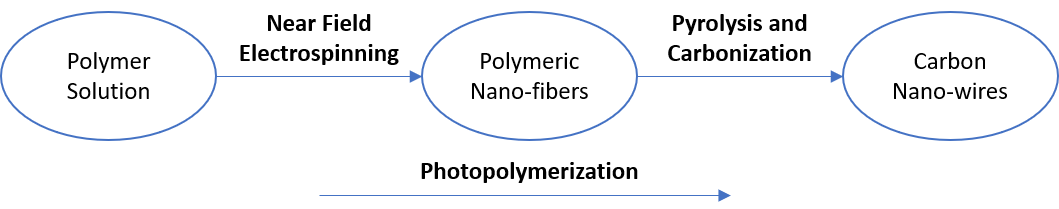
\includegraphics[width=0.95\textwidth]{./Figures/FabricationProcess.png}
%\decoRule
%\caption[Carbon Nano-wires Fabrication Process]{Fabrication process of carbon nano-wires to achieve through the proposed dissertation.}
%\label{fig:fabricationFlowChart}
%\end{figure}

%\begin{equation}
%\left(\tau _t^e-\frac{\tau _n^e \text{dr}}{\text{dz}}\right) 2 \pi  r+\frac{d \left(\pi  r^2
%   \left(\tau _{\text{zz}}-p\right)\right)}{\text{dz}}+\frac{\gamma  \text{dr} 2 \pi  r}{r
%   \text{dz}}+\rho  g \pi  r^2=\frac{d \left(\rho  \pi  r^2 v^2\right)}{\text{dz}}
%\label{eq:linearMomentum}
%\end{equation}